\begin{titlepage}
	\begin{center}
		\chapter{Introduction}
		\minitoc

		\vspace{5cm}
		\pgfspectra[element=He,absorption]
	\end{center}
	\vfill % Remplir le reste de la page avec du blanc
\end{titlepage}
\pagestyle{monstyle}\setcounter{page}{1}

\section{Historique}
\subsection{1950}
\compo[0.8]{
    ce concept existe depuis des décennies mais, jusqu'en 1950, les
    gens ignoraient le terme. John McCarthy, connu comme le
    fondateur de l'intelligence artificielle, a introduit le terme
    ``intelligence artificielle'' en 1955, avec l'objectif de faire
    produire des tâches humaines par des machines mimant l'activité du
    cerveau.
}{
    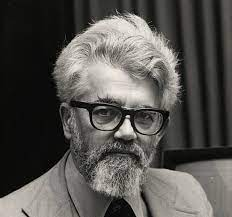
\includegraphics[height=\textwidth,width=\textwidth]{photo/jon_maccrthy.jpg}
}
\subsection{1970}
\compo[0.8]{
    les scientifique ont pris fin à création de tous les algorithmes
    d'intelligence artificiels, mais la puissance des ordinateurs sont très
    faibles

}{
    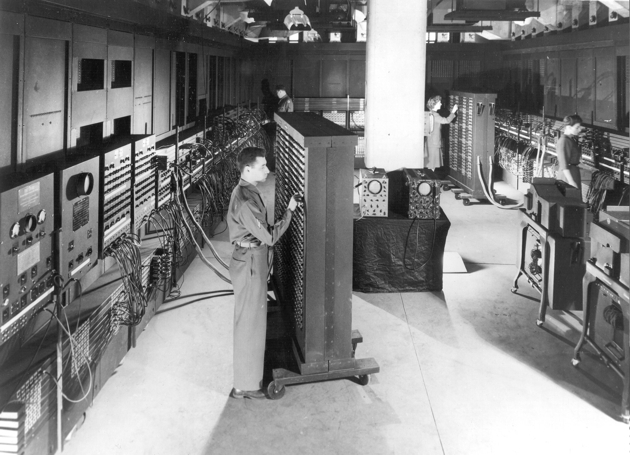
\includegraphics[height=\textwidth,width=\textwidth]{photo/1970.jpg}
}
\subsection{1980}
\compo[0.6]{
    développement des réseaux de neurones artificiels, grâce à l'augmentation
    de puissance des ordinateurs et à l'accumulation des gigantesques quantités
    de données(big data).

    Par le biais d’un algorithme, le réseau de neurones artificiels
    permet à l’ordinateur d’apprendre à partir de nouvelles données.
    L’ordinateur doté du réseau de neurones apprend à effectuer une
    tâche en analysant des exemples pour s’entraîner. Ces exemples ont
    préalablement été étiquetés afin que le réseau puisse savoir ce
    dont l s’agit.

    Par exemple, un réseau de neurones peut être utilisé pour
    apprendre à l’ordinateur à reconnaître des objets. Un grand nombre
    d’objets d’une même catégorie est présenté au réseau de neurones,
    et l’ordinateur apprendre à reconnaître cet objet sur de nouvelles
    images en analysant les patterns récurrentes au sein des images
    d’exemple. Ainsi, en analysant des milliers de photos de chats, le
    Neural Network apprendra à reconnaître un chat sur n’importe
    quelle photo.
}{
    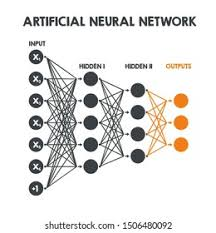
\includegraphics[height=\textwidth,width=\textwidth]{photo/neuron.jpg}
}

\subsection{Premier applications dans la médecine}
    développement des réseaux de neurones artificiels, grâce à l'augmentation
    de puissance des ordinateurs et à l'accumulation des gigantesques quantités
    de données(big data).

\subsection{les dizaine année dernier}
    Google AI mis au point une \textbf{IA} qui prédit le cancer du poumon avec
    $94,4~\%$ de réussite. Ces procédures empêchent également les tests invasifs comme les biopsies.
    L'IA apporte également une aide à la prescription, par exemple
    en détectant automatiquement un risque d'allergie ou
    d'interaction médicamenteuse.

\section{Définition}
\compo[0.8]{
    \begin{itemize}
        \item
            Les algorithmes de \textbf{IA} est basé sur  l'injections des milliards de données
            dans un programme d'apprentissage,

        \item
            dans le cas des algorithmes du médecine, on apprend à ``reconnaître'' les signes
            de la maladie.
    \end{itemize}
}
{
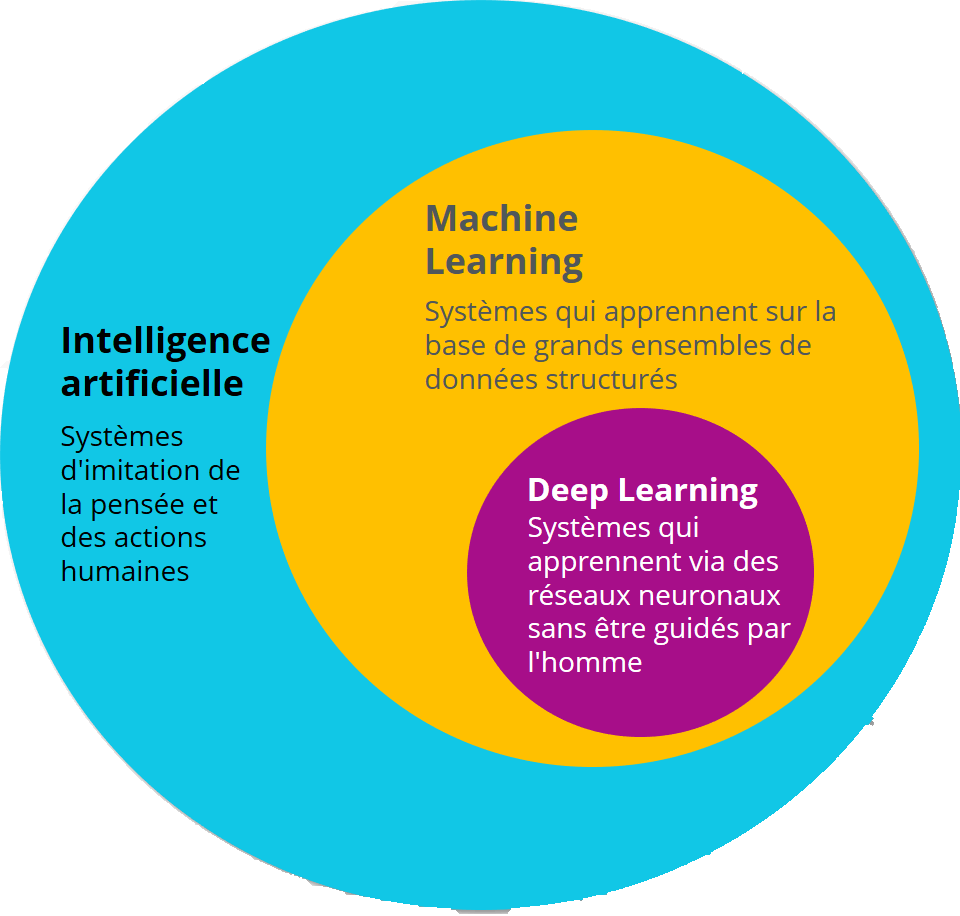
\includegraphics[height=\textwidth,width=\textwidth]{photo/ai1a.png}
}


\subsection{Machine Learninig}
\begin{itemize}
    \item
    ``Machine learninig'' apprentissage automatique, une méthode fondée sur
    la représentation mathématique et informatique de neurones
    biologiques, selon des modalités plus ou moins complexes.

    \item
    Les algorithmes d'apprentissage profond (deep learning) par exemple, dont
    l'usage explose depuis une dizaine d'années, font une analogie
    lointaine avec le fonctionnement cérébral en simulant un réseau de
    neurones organisés en différentes couches, échangeant les uns avec les
    autres.

    \item
    La force de cette approche est que l'algorithme apprend la
    tâche qui lui a été assignée par ``essais et erreurs''.
\end{itemize}
\subsection{Deep Learning}
    Utilisation des algorithmes d'intelligence artificielle pour permettre
    en quelque sorte aux ordinateurs d'apprendre par eux-mêmes On
    appelle cela l'apprentissage profond ou ``deep learning'' en anglais.

\section{Des applications}
\begin{itemize}
    \item
        l'application de \textbf{IA} en traitement d'images, par exemple pour repérer de
        possibles mélanomes sur les photos de peau, ou bien pour dépister des
        rétinopathies diabétiques sur des images de rétines. Leur mise au point
        nécessite de grands échantillons d'apprentissage.
    \item
        en prend plus de 50 000 images dans le cas des mélanomes, et 128 000
        dans celui des rétinopathies, ont été nécessaires pour entraîner
        l'algorithme à identifier les signes de pathologies. Pour chacune
        de ces images on lui indique si elle présente ou non des signes
        pathologiques.
    \item
        A la fin de l'apprentissage, l'algorithme arrive à
        reconnaître avec une excellente performance de nouvelles images
        présentant une anomalie.
\end{itemize}

\section{Les conditions pour utilisée IA}
\begin{itemize}
    \item Les experts:
            les procédures interventionnelles demandent une dextérité
            manuelle et un sens commun pour s'adapter à des situations changeantes.
        
    \item IA:
            Le travail des médecins radiologistes comprend de nombreuses tâches,
            dont les plus rapides comme la détection d'une anomalie ou les plus
            répétitives comme les mesures se prêtent bien à l'automatisation.\mybox
        
\end{itemize}
